\chapter{El TNS y la red mundial de observatorios}
Entender el mecanismo de aceleración de partículas es un tema trascendental en la astrofísica, más aún el proceso de aceleración de iones que todavía no se comprende perfectamente. El Sol, siendo el acelerador natural de partículas más cercano, provee de grandes oportunidades para estudiar este proceso\cite{ValdesGalicia2009565}. El mejor camino para entender el mecanismo de aceleración de iones en la atmósfera solar es usando datos obtenidos por los detectores de neutrones y rayos gama\cite{murak}.\\

Los monitores de neutrones tienen cuentas muy elevadas debido a su alta sensibilidad y no pueden diferenciar la dirección de arribo de las partículas incidentes\cite{Tsuchiya2001183}. Tampoco resuelven la energía de las partículas y no discriminan entre neutrones y protones. Por esta razón, es necesario el uso de un nuevo equipo para resolver los inconvenientes mencionados. El Telescopio de Neutrones Solares \textsc{(TNS)} puede diferenciar entre neutrones y protones, y medir el flujo neutrones solares, su energía y dirección de arribo de las partículas incidentes\cite{valdes,TNS}.\\

En este capítulo se muestra la red mundial de Telescopios de Neutrones Solares y se describen las carácteristicas del TNS instalado en Sierra Negra, así como la estructura de los datos registrados. \\

\section{Red mundial de TNS}

Para interpretar cualquier medición de intensidad de radiación cósmica que se realice cerca de la superficie de la tierra se requiere tomar en cuenta la presencia del campo magnético terrestre. El campo geomagnético, así como nos protege de los efectos nocivos, también controla la cantidad de rayos cósmicos que llega a la superficie. Por ejemplo, si apuntamos un detector de rayos cósmicos hacia la dirección vertical, se observará que el detector recibe todas las partículas de rigideces altas, como si no estuviera el campo geomagnético. Sin embargo, si seguimos midiendo el flujo de rigideces magnéticas menores veremos que hay una rigidez debajo de la cual ya no se detecta ninguna partícula, a ésta se le conoce como \emph{rigidez umbral}. Además, si desplazamos el detector vertical desde el ecuador hacia los polos veremos que la rigidez umbral va disminuyendo\cite{mensajeros}. De este modo, los rayos cósmicos que llegan a mayores latitudes magnéticas penetran facilmente a la atmósfera, mientras que los que llegan a bajas latitudes magnéticas requieren más energía para penetrar.\\

Además de la latitud geomagnética y la energía de partículas, la altura a la cual se encuentra el detector también es muy importante; si se ubica a grandes alturas sobre el nivel del mar, el número de cuentas que registre será mayor debido a que la absorción atmosférica de las partículas secundarias disminuye pues hay menos masa\cite{chismes}.\\

Si se quiere tener una mayor eficiencia en la detección de neutrones, los telescopios deben ser colocados muy cerca del ecuador para que el tiempo de exposición a la radiación solar sea más uniforme a lo largo del año y que la rigidez umbral requerida para los iones incidentes sea muy alta. También debe estar localizado a la mayor altura posible para reducir la cantidad de materia que puede interaccionar con los neutrones solares, disminuyendo la posible contaminación de partículas energéticas cargadas. Por lo tanto, los sitios ideales para las mediciones es en lo alto de las montañas.\\

Predecir cuándo habrá un evento de neutrones solares es imposible, por ello se ha instalado una red de telescopios de neutrones solares a diferentes longitudes alrededor del mundo para tener observación del Sol las 24 horas. La red mundial de TNS está construida tomando en cuenta los detalles sobre la localización geográfica para tener una óptima observación. Hasta ahora se han instalado siete detectores de este tipo alrededor del planeta, el más nuevo de ellos es el instalado en México. En la figura \ref{red} se puede ver la localización geográfica de cada TNS, así como el país en el que se encuentra instalado.\\


\begin{figure}[H]
  \centering
    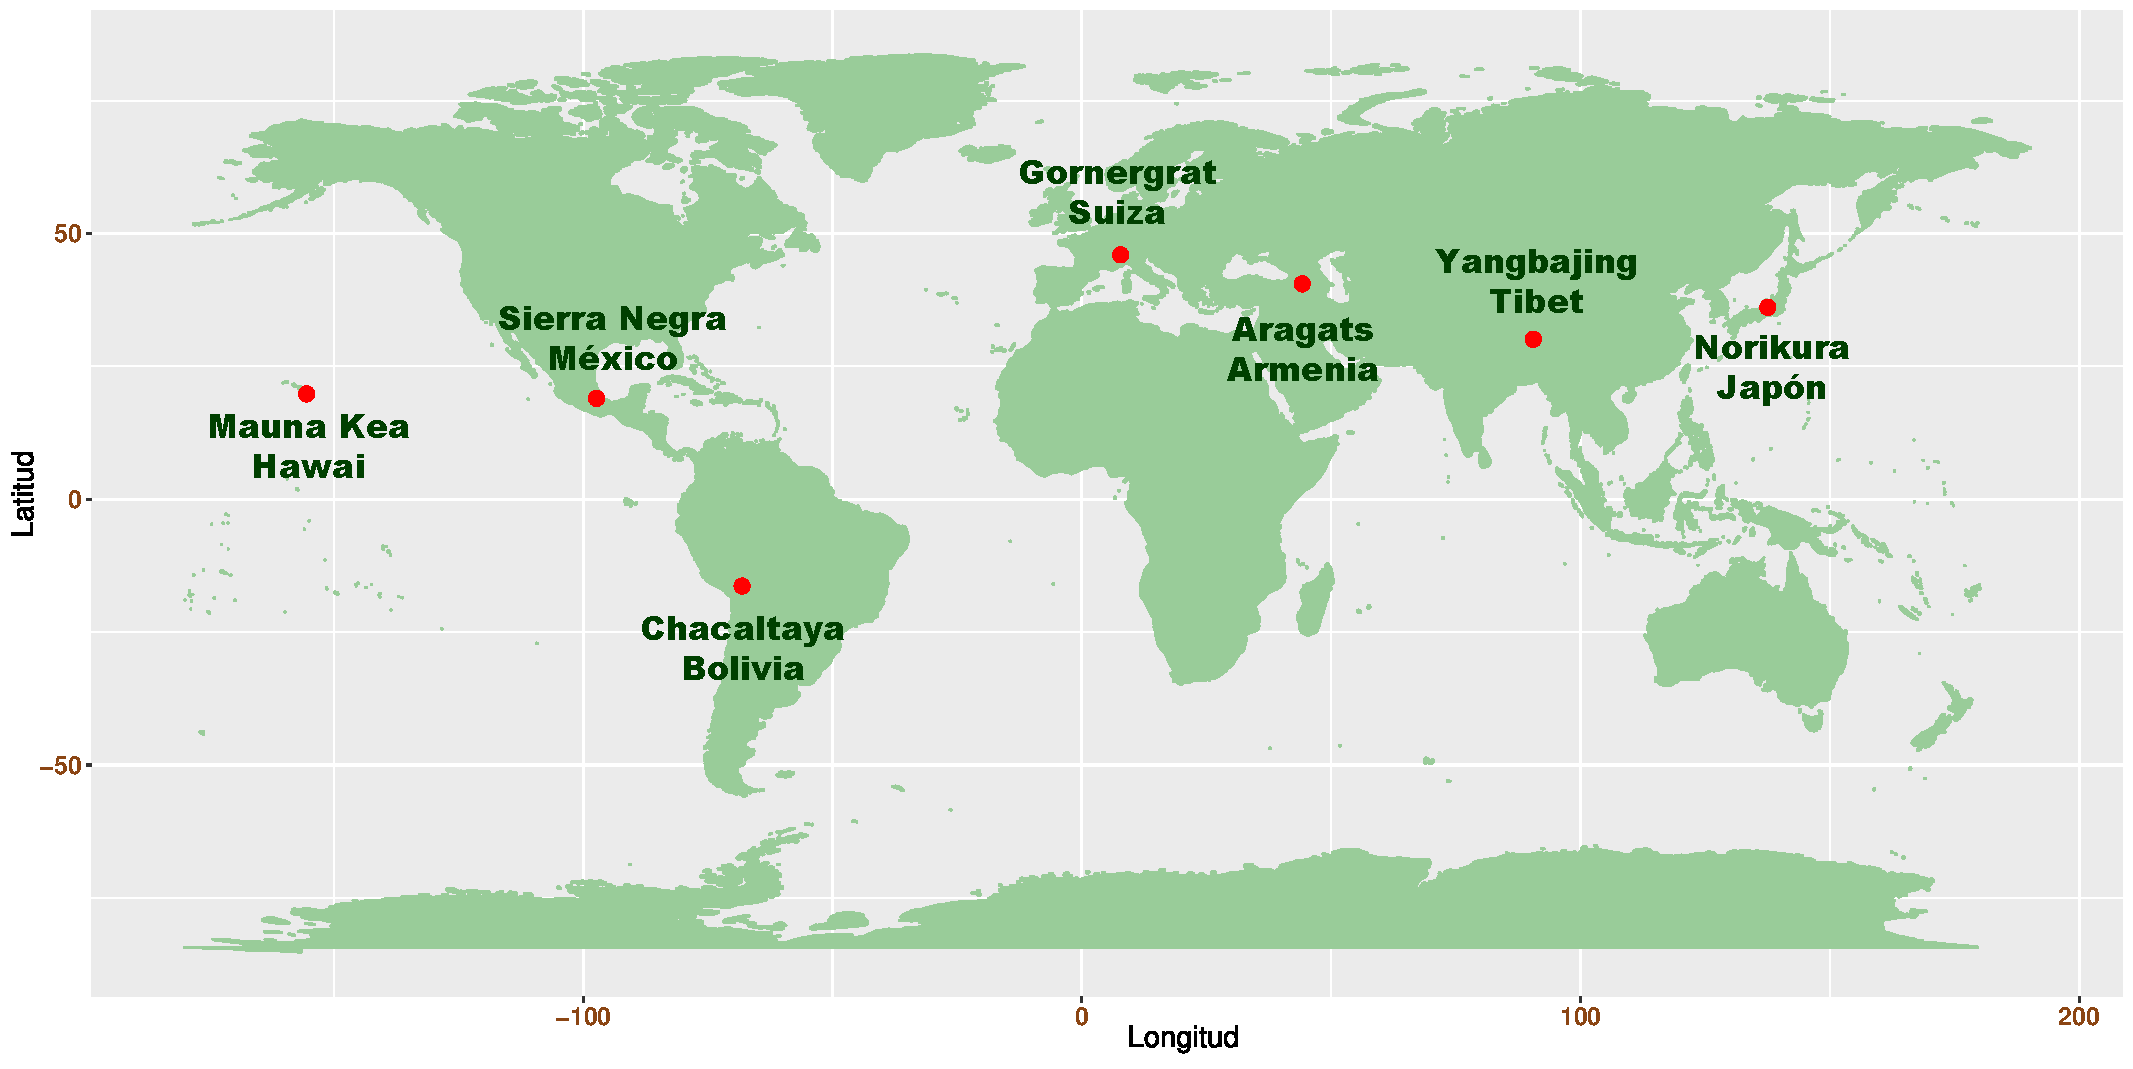
\includegraphics[scale=0.43]{Capitulo2/figs/mapatns.pdf}      %Ruta completa de la imagen, porque se compila desde el archivo tesis.tex
  \caption{Localización geográfica de los TNS alrededor del planeta.}            %Pie de imagen
  \label{red}                            %nombre de referencia
\end{figure}


En la tabla \ref{caractred} se  muestra las coordenadas y altura de los siete TNS  que conforman la red mundial, también la fecha en que se comenzaron a hacer las primeras observaciones. Para ver más características de los TNS se recomienda \textit{Detection efficiency of a new type of solar neutron detector calibrated by an accelerator neutron beam} de H. Tsuchiya \cite{Tsuchiya2001183}.\\

\begin{table}[htb]
\centering
\begin{tabular}{|c|c|c|c|c|}
\hline
{\bf \multirow{2}{*}{Localización}}  & \multirow{2}{*}{{\bf Altura}} & {\bf \multirow{2}{*}{ Longitud}} & {\bf \multirow{2}{*}{Latitud}} & {\bf \multirow{2}{*}{Inicio de la }}\\
  & m.s.n.m &  &  & \bf observación \\
\hline
Gronergrat, Suiza  & 3135 &  $7.8^{\circ}$ E & $46.0^{\circ}$ N & Enero 1998\\
\hline
Aragats, Armenia  & 3200 & $40.5^{\circ}$ E & $44.2^{\circ}$ N & Jun 1997\\
\hline
Yanbajing, Tibet  & 4300 & $90.5^{\circ}$ E & $30.0^{\circ}$ N & Sep 1998\\
\hline
Mt. Norikura, Japón  & 2770 & $137.5^{\circ}$ E & $36.1^{\circ}$ N & Oct 1990\\
\hline
Mauna Kea, Hawaii  & 4200 & $156.3^{\circ}$ W & $19.8^{\circ}$ N & Abr 1997\\
\hline
Sierra Negra, México  & 4580 & $97.3^{\circ}$ W & $19.0^{\circ}$ N & Jul 2004\\
\hline
Chacaltaya, Bolivia & 5250 & $68^{\circ}$ W & $16.2^{\circ}$ S & Sep 1992\\
\hline
\end{tabular}
\caption{Datos de la Red Mundial de TNS.} 
\label{caractred} 
\end{table}

\section{El TNS en Sierra negra}

Sierra Negra es un volcán inactivo localizado en la parte oriental del estado de Puebla, tiene una altura de 4580 m s.n.m., es uno de los picos más altos de la meseta central mexicana. La cima del volcán alberga diversos proyectos astronómicos,\footnote{El Observatorio Solar Mexicano de Gran Altura (OSOMEGA) de la Universidad Nacional Autónoma de México (\url{http://naolinco.geofisica.unam.mx/observatorios/osmega/index.html}). También el Gran Telescopio Milimétrico, un proyecto entre el Instituto Nacional de Astrofísica, Óptica y Electrónica (INAOE) y la Universidad de Massachusetts Amherst (\url{http://www.lmtgtm.org/?lang=es}), entre otros.} uno de ellos es el TNS que forma parte de la red mundial de observatorios.\\

Debido a su localización geográfica, Sierra Negra fue escogido como el mejor lugar para colocar un TNS en México. Además, las condiciones atmosféricas son lo suficientemente moderadas; así que se preserva el flujo de una buena parte de neutrones solares emitidos en fulguraciones. La instalación se llevó a cabo entre el STELab (Solar Terrestrial Environment Laboratory) de la Universidad de Nagoya, Japón y el Instituto de Geofísica de la UNAM.\\

Se puede ver en la figura \ref{red} que el TNS en Sierra Negra está ubicado, longitudinalmente, entre los detectores de Hawai y Chacaltaya, lo cual ayuda a tener en observación al Sol de manera continua, y la combinación de altura/latitud proporciona un tiempo considerable para tal efecto .\\

El TNS fue construido y probado en Marzo de 2003 en Sierra Negra, Puebla ($97.3^{\circ}$ W, $19.0^{\circ}$ N) y ha estado operando desde julio de 2004\cite{geo}. La figura \ref{tns} muestra un esquema del TNS.\\
 
 \begin{figure}[H]
  \centering
    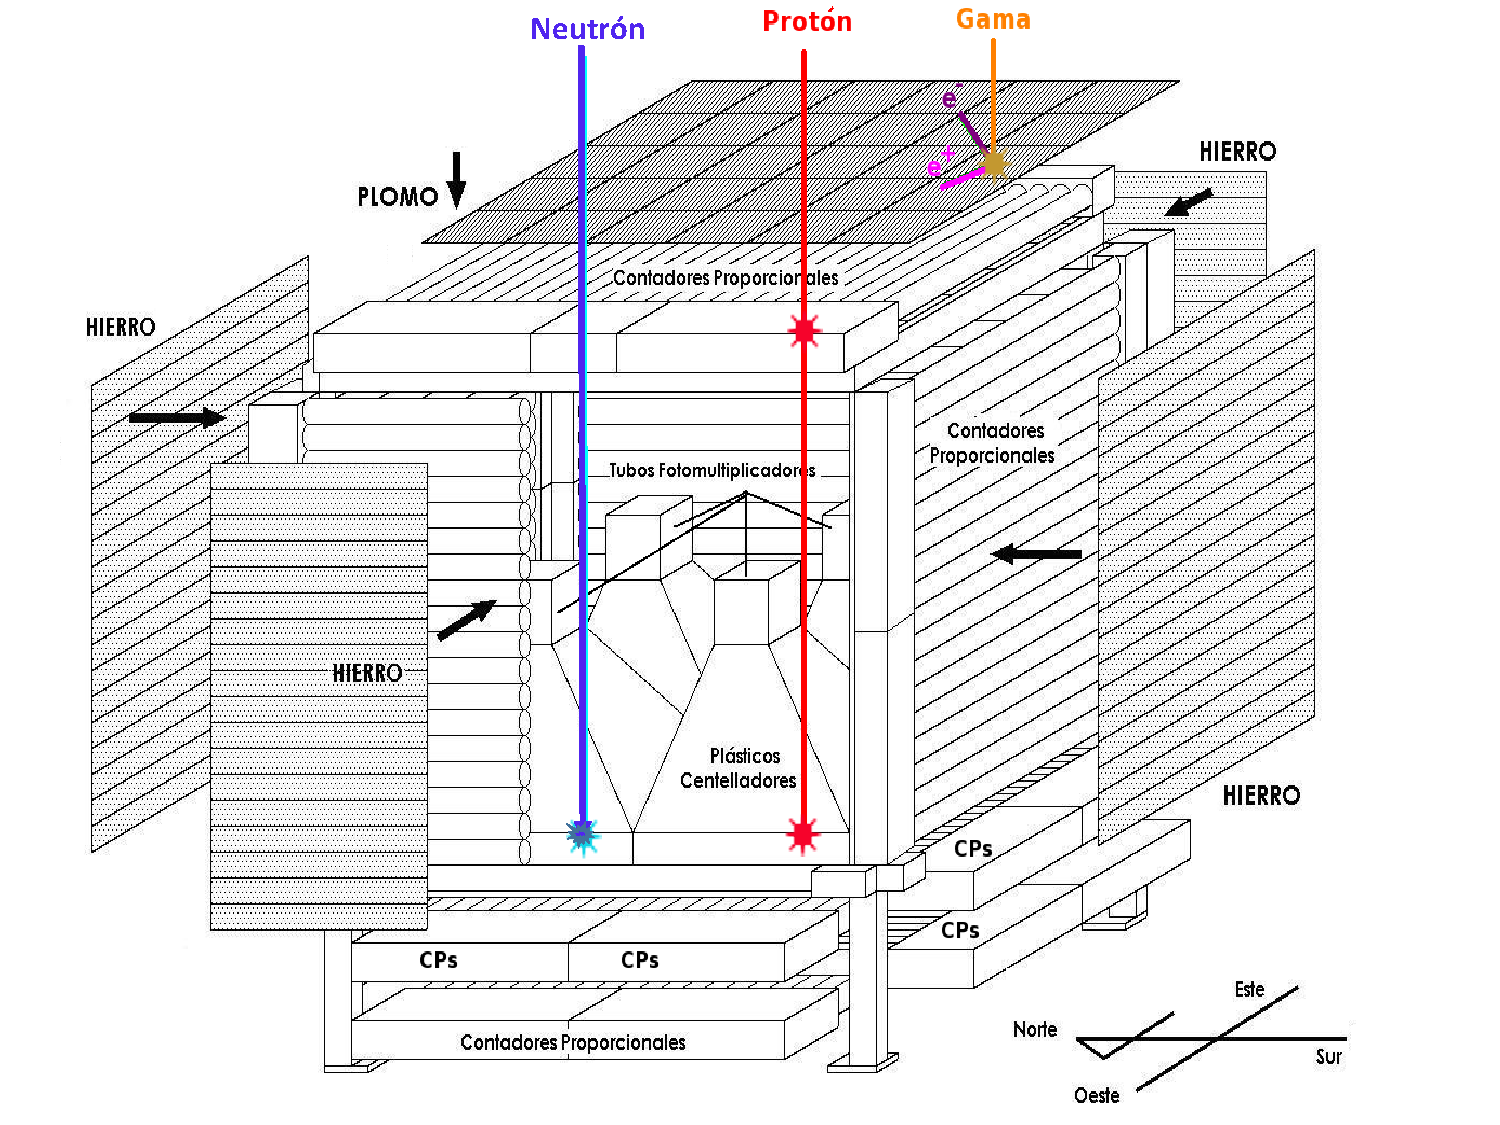
\includegraphics[scale=0.60]{Capitulo2/figs/EsTNS.pdf}      %Ruta completa de la imagen, porque se compila desde el archivo tesis.tex
  \caption{Esquema del TNS instalado en la cima del volcán Sierra Negra, Puebla.}            %Pie de imagen
  \label{tns}                            %nombre de referencia
\end{figure}

El TNS en Sierra Negra consiste de 4 plásticos centelladores (PC) con área de $1m^2$ cada uno y espesor de 30cm; así el área total de detección es de $4m^2$. Los PC están rodeados por arreglos de contadores proporcionales (CP).\\

Se diferencía entre partículas neutras y partículas cargadas mediante un sistema de anticoincidencias electrónicas entre la señal que disparan los PC y CP. Es decir, las partículas cargadas dejan señal en los plásticos centelladores y en los contadores proporcionales; mientras que las partículas neutras lo hacen sólo en los plásticos centelladores.\\

La energía depositada por las partículas incidentes se mide en un tubo fotomultiplicador instalado arriba de cada PC, la altura del pulso obtenido por cada fotomultiplicador se discrimina en 4 diferentes canales de deposición de energía; $E\geq 30 \, MeV$ ($S1 \_ with \_ anti$), $E\geq 60 \, MeV$ ($S2 \_ with \_ anti$), $E\geq 90 \, MeV$ ($S3 \_ with \_ anti$), $E\geq 120 \, MeV$ ($S4 \_ with \_ anti$).\\

Por encima de los CP se colocó una placa de 0.5 cm de espesor de Plomo; por los lados, los  CP se protegieron con placas de Hierro de 0.5 cm de espesor. Estas placas sirven para reducir la radiación de fondo, ya que los fotones muy energéticos pueden dejar una señal similar a la de los neutrones. \\

Las direcciones de arribo se miden usando cuatro capas de CP alineados ortogonalmente debajo de los PC, dos para determinar la dirección de arribo E-W y dos más para la dirección N-S. Estas direcciones, N-S y E-W están divididas en cinco secciones, con lo cual se tienen 25 canales de dirección. Las direcciones se determinan usando los protones producidos por los neutrones al interaccionar con los PC. Estos protones secundarios se desvian menos de $13.48^{\circ} $ de su dirección original con lo que se asegura que la dirección de arribo del neutron puede ser determinada\cite{TNS}.\\

Hasta aquí se ha visto de qué forma el TNS diferencia entre partículas cargadas y partículas neutras, la manera en que se mide la energía de las partículas, su dirección de arribo y el flujo de partículas neutras. Después de esto, es importante saber si la capacidad de detección del TNS es adecuado, es decir,  que las mediciones de neutrones solares son correctas y que no está contaminado por otras partículas.\\

La eficiencia de detección de los detectores de neutrones solares se calcula mediante una simulación Monte Carlo. El TNS en Sierra Negra tiene una capacidad de detección del 10 \%, para neutrones solares muy energéticos, tomando en cuenta los plásticos centelladores. Sin embargo, la eficiencia disminuye si se toma en cuenta los contadores proporcionales y las placas de Hierro y Plomo. En \textit{El Telescopio de Neutrones Solares en Sierra Negra y Aceleración de Iones en la Atmósfera Solar} de Luis Xavier González\cite{TNS} se pueden ver los detalles de la capacidad de detección del TNS  tomando en cuenta los componentes mencionados.\\

Una vez que el TNS en Sierra Negra estuvo instalado y probado se empezaron a registrar las primeras observaciones en julio de 2004. Despues de 13 años de detección es conveniente estudiar la estabilidad de los datos para distinguir las diferentes variaciones. Para ello es importante conocer la estructura de los datos registrados antes de procesarlos y así saber cómo manipularlos.


\section{Datos del TNS en Sierra Negra}

Es de gran importancia analizar los datos del TNS para tener un resumen de las variaciones que ha presentado su desempeño a lo largo del tiempo. El análisis se realiza para los cuatro canales de deposición de energía que registran partículas neutras, se registra como anti-coincidencia electrónica ($S\_with\_anti$).\\
 
 El registro de la detección se guarda en un archivo diario, cada archivo se almacena en la carpeta del mes correspondiente y, a su vez, la carpeta de cada mes en el año correspondiente. El nombre con el que se guarda el archivo es la fecha del día con extensión \textbf{sn1} si no hubo ninguna suspensión en el registro, de lo contrario se generan $i$ archivos con extensión sn$j$ (donde $j=1,...,i$) para $i-1$ interrupciones. La ventaja de este tipo de extensión es que los datos se pueden visualizar en cualquier editor de textos y datos en ascii.\\

La razón de conteo desde enero de 2004 al 6 de marzo de 2006 fue de 1 minuto, y a partir del 8 de Marzo de 2006 los registros se hicieron cada 10 segundos. Excepto del 5 de marzo de 2008 al 24 de abril de 2008 que fue de 3 segundos.\\
 
Debido a fallas electrónicas en el equipo periférico y de suministro de energía eléctrica hay muchos archivos en los que se suspendió el registro por algunas horas, otros en los que se registraron datos de 0 en todo el día y días en los que no se registró la detección del TNS. Para esto se tomó nota de los archivos completos (registro de las 24 horas), de los que se suspendieron y la hora en que sucedió, para los años 2004 hasta 2016.\\

Durante todo el año del 2007 el TNS estuvo desconectado. Así, desde 2004 a 2016 no hay registros de 1205 días. La figura \ref{detec} muestra el número de días registrados por cada mes y año. Con esta gráfica se puede observar fácilmente en qué meses hay pocos registros.\\

 \begin{figure}[H]
  \centering
    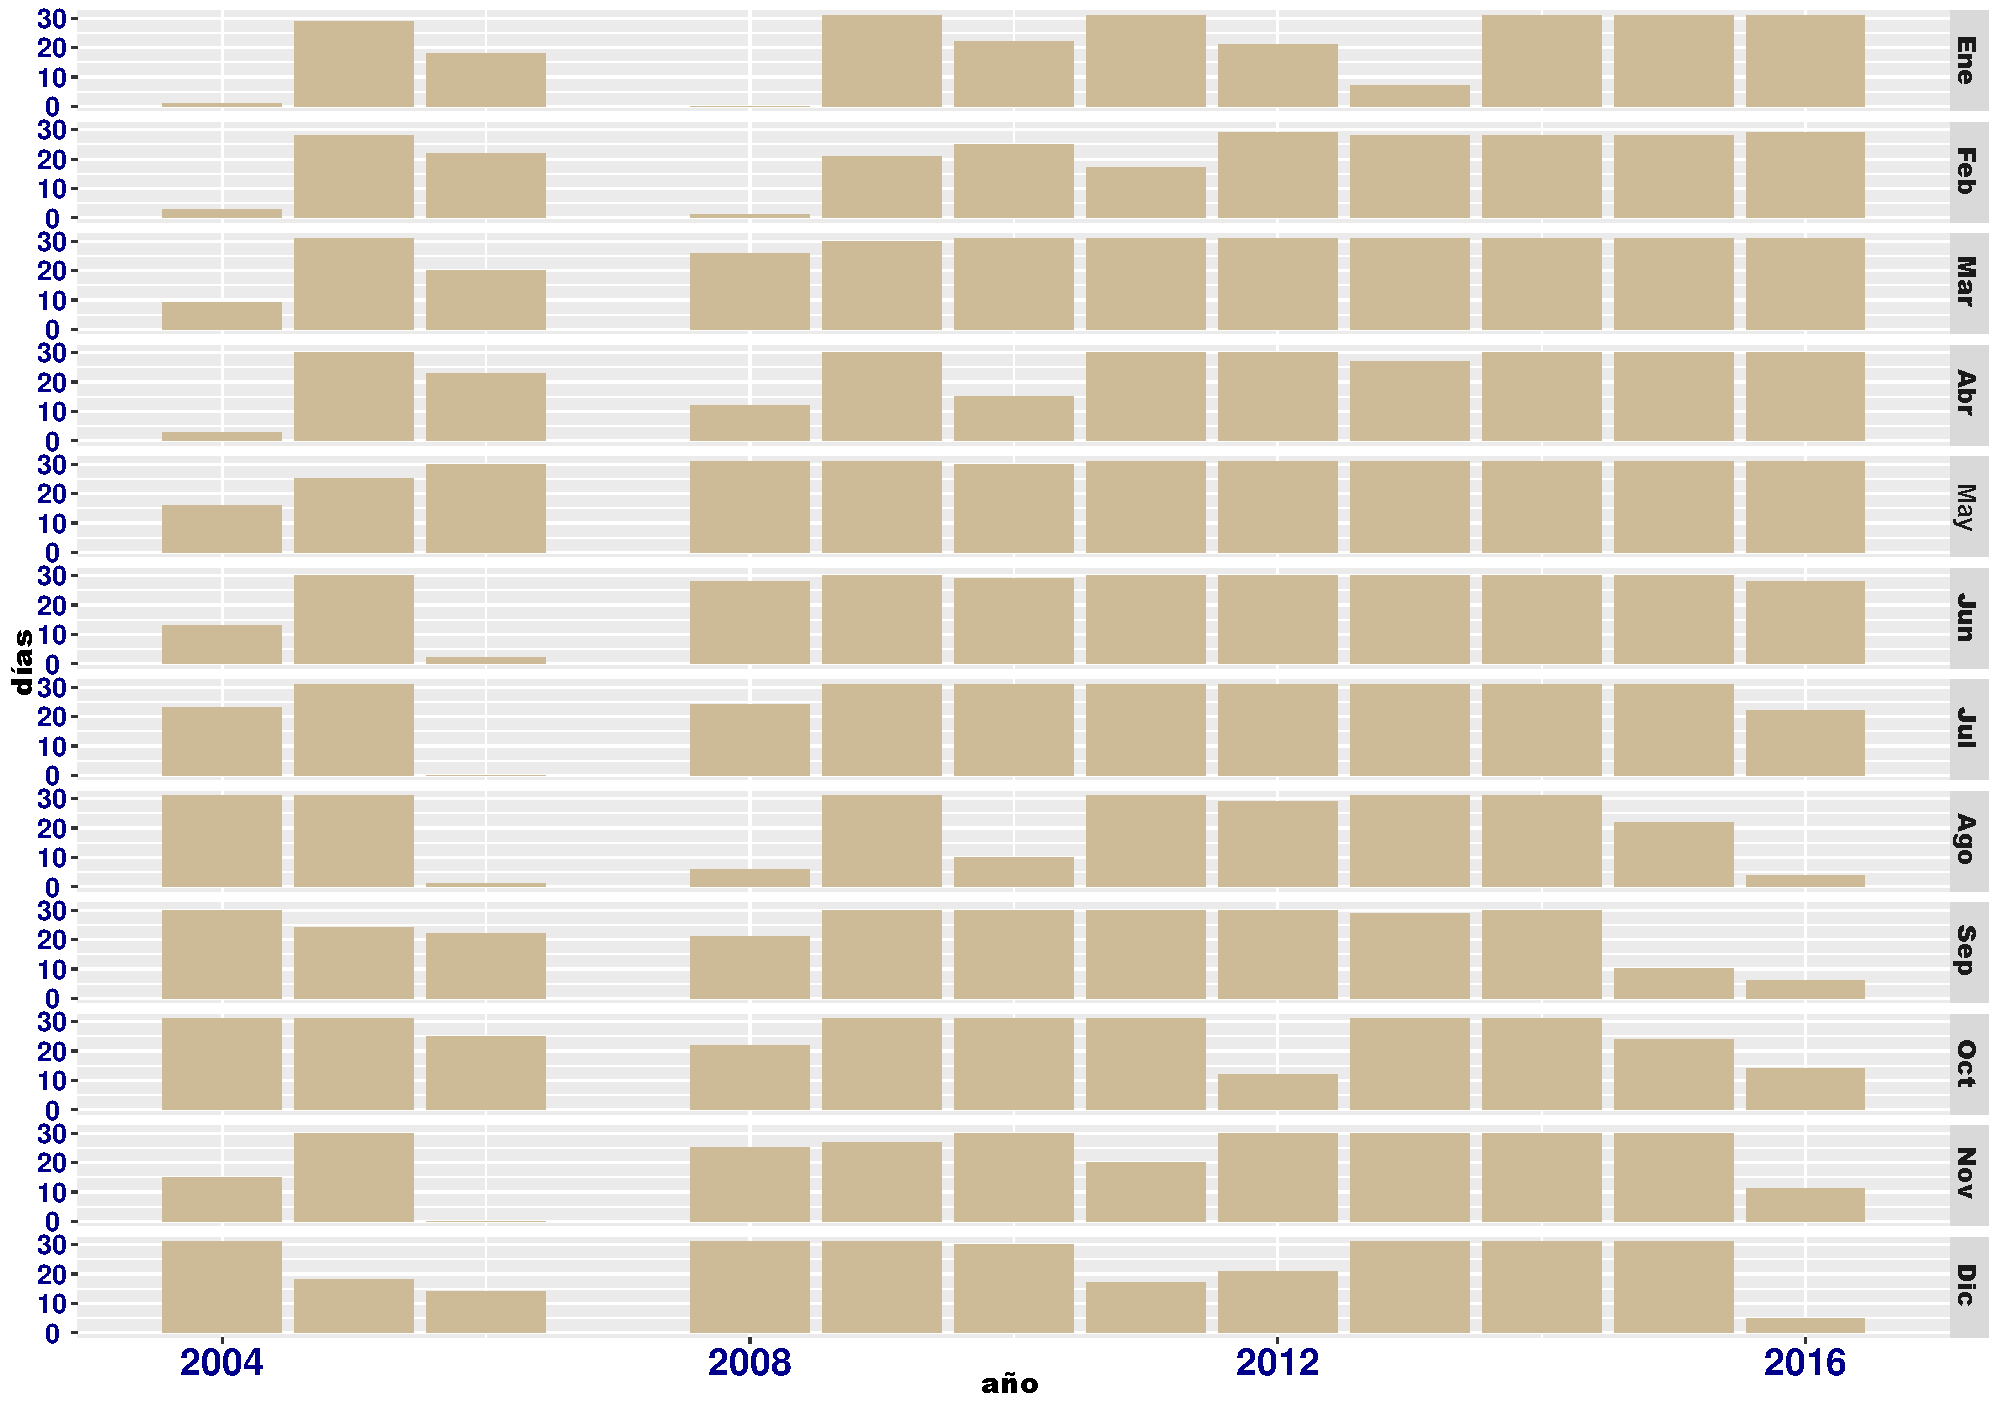
\includegraphics[scale=0.45]{Capitulo2/figs/detectados.pdf}      %Ruta completa de la imagen, porque se compila desde el archivo tesis.tex
  
  \caption{Gráfica que muestra el número de días registrados por mes y año.}            %Pie de imagen
  \label{detec}                            %nombre de referencia
\end{figure}

Es importante destacar que la gráfica sólo muestra la cantidad de días en que hubo registros, lo cual no quiere decir que todos los datos registrados sean ``buenos". Por ejemplo, en abril del 2010 hubo varios cortes de energía que duraron más de un día. Así varios archivos no tienen datos, los datos son constantes o los archivos están interrumpidos porque el soporte de energía era de 18 horas y el corte respectivo fue mayor.\\
  
También en septiembre de 2010, varios días tienen datos con ceros, debido a cortes en el suministro de energía eléctrica. Este problema persistió hasta principios de 2011. En el \emph{capítulo 3} se mostrará el porcentaje de datos confiables.\\

\section{Estructura de archivos registrados}

Antes de pasar al siguiente capítulo para mostrar los códigos usados al importar los datos, es necesario conocer cómo están estructurados. Se han manejado varias razones de conteo: de 3 segundos, 10 segundos y un minuto.\\

En la Tabla \ref{min} se muestran las primeras y últimas filas del archivo mx040720.sn1, que contiene datos del 20 de julio de 2004. La primera columna denota el año en que se está llevando a cabo el registro, en este caso 2004; la segunda columna contiene el número del mes y el día, es decir, 720 indica que es el día 20 del mes 7 (julio). En la columna 3 se encuentra el tiempo, empieza con el minuto 0, sigue el minuto 1, 2, 3 , 4 hasta llegar al minuto 59 y luego 100 que denota la hora 1 con cero minutos. Se sigue con 101,102 hasta llegar a 159, luego 200, que es la hora 2 con cero minutos. De esta manera, llega a la fila 1440 a la hora 23 con 59 minutos y termina con el minuto 0 del siguiente día.\\

La cuarta columna no es ningún dato relevante. De la columna 5 a la 8 son los datos de partículas neutras (canales S1\_A, ..., S4\_A), de la columna 9 a la 12 son datos de partículas cargadas desde S1 hasta S4. Luego siguen otras 378 columnas con registro de otros datos que no se usarán para este trabajo.\\  


\begin{table}[H]
  \centering
\centering
\begin{tabular}{r|cccccccccccc}
  & 1 & 2 & 3 & 4 & 5 & 6 & 7 & 8 & 9 & 10 & 11 & $\cdots$ \\
  \hline
1 & 2004 & 720 &   0 & 100 & 8761 & 3407 & 1196 & 541 & 27371 & 12855 & 5036 & $\cdots$\\ 
  2 & 2004 & 720 &   1 &   0 & 8602 & 3355 & 1187 & 539 & 27619 & 13003 & 5083 & $\cdots$\\ 
  3 & 2004 & 720 &   2 &   0 & 8705 & 3402 & 1261 & 580 & 27804 & 13205 & 5194 & $\cdots$\\ 
  4 & 2004 & 720 &   3 &   0 & 8662 & 3400 & 1235 & 565 & 27645 & 12987 & 5051 & $\cdots$\\ 
  5 & 2004 & 720 &   4 &   0 & 8712 & 3323 & 1178 & 551 & 27702 & 12876 & 4994 & $\cdots$\\ 
  6 & 2004 & 720 &   5 &   0 & 8642 & 3271 & 1210 & 553 & 27627 & 12857 & 5107 & $\cdots$\\ 
$\vdots$ & $\vdots$ & $\vdots$ & $\vdots$ & $\vdots$ & $\vdots$ & $\vdots$ & $\vdots$ & $\vdots$ & $\vdots$ & $\vdots$ & $\vdots$ &  \\
  1436 & 2004 & 720 & 2355 &   0 & 8577 & 3316 & 1204 & 569 & 27647 & 13057 & 5104 & $\cdots$\\ 
  1437 & 2004 & 720 & 2356 &   0 & 8652 & 3358 & 1233 & 561 & 27647 & 12928 & 5083 & $\cdots$\\ 
  1438 & 2004 & 720 & 2357 &   0 & 8665 & 3400 & 1231 & 545 & 27596 & 12999 & 5039 & $\cdots$ \\ 
  1439 & 2004 & 720 & 2358 &   0 & 8732 & 3399 & 1226 & 548 & 27675 & 12983 & 5060 & $\cdots$\\ 
  1440 & 2004 & 720 & 2359 &   0 & 8681 & 3355 & 1152 & 557 & 27789 & 12983 & 5009 & $\cdots$\\ 
  1441 & 2004 & 721 &   0 &   0 & 8651 & 3377 & 1252 & 558 & 27848 & 13032 & 5098 & $\cdots$\\ 
  
\end{tabular}

\caption{Datos del 20 de julio de 2004, razón de conteo de 1 minuto.}
\label{min}     
\end{table}


Ahora véase la Tabla \ref{10seg}, con datos del 1 de junio de 2008, esta es la estructura de los archivos registrados cada 10 segundos. Las primeras cinco filas contienen información acerca del registro de ese día, como \emph{INTERVAL} que indica el intervalo de tiempo entre cada observación, \emph{DATE}  contiene la fecha en el formato año, mes y día (080601, 1 de junio de 2008). TIME es la hora o tiempo en que empieza el registro, en este caso 000000 indica que empieza a las 0 horas, 0 minutos con 0 segundos. Mientras que la última fila ( fila 8646) dice que el archivo termina con 8640 observaciones.\\

Como se puede ver, las primeras cinco filas son innecesarias, ya que la columna 2 contiene la fecha en el mismo formato para cada observación, así como la columna 3 guarda la hora, minuto y segundo. De la columna 4 a la 7 son datos de partículas neutras (canales S1\_A, ..., S4\_A), mientras que la columna 8 a la 11 guarda datos de partículas cargadas (S1, ..., S4). En total el archivo contiene 52 columnas.\\


\begin{table}[H]
  \centering
\begin{tabular}{r|llccccccccc}
  & 1 & 2 & 3 & 4 & 5 & 6 & 7 & 8 & 9  & $\cdots$\\
\hline

 1 & NCHANNEL &         48 &        &      &     &   &    &  &  &       \\

 2 & INTERVAL &         10 &        &        &      &      &    &  & &   \\

 3 & VERSION &       3.00 &        &       &       &      &     &  & &       \\

 4 & DATE &      080601 &        &         &       &      &    &    & &      \\

 5  & TIME &      000000 &        &        &       &      &   &   & &     \\

  6 & SG & 080601 & 000010 & 12400 & 4120 & 1108 & 108 & 26692 & 11292  & $\cdots$\\ 
  7 & SG & 080601 & 000020 & 12408 & 4100 & 1036 &  12 & 26656 & 11372  & $\cdots$\\ 
  8 & SG & 080601 & 000030 & 12364 & 4124 & 1104 & 104 & 26636 & 11344  & $\cdots$\\ 
  9 & SG & 080601 & 000040 & 12292 & 4108 & 1024 & 124 & 26664 & 10292 & $\cdots$\\ 
  10 & SG & 080601 & 000050 & 12348 & 4216 & 1148 &  60 & 26632 & 11364 & $\cdots$\\ 
  11 & SG & 080601 & 000100 & 12412 & 4188 & 1028 &   0 & 26740 & 10260 & $\cdots$\\ 
  $\vdots$ & $\vdots$ & $\vdots$ & $\vdots$ & $\vdots$ & $\vdots$  & $\vdots$ & $\vdots$ & $\vdots$ & $\vdots$ &  \\
  8641 & SG & 080601 & 235920 & 12408 & 4108 & 1136 &   4 & 26704 & 10316 & $\cdots$\\ 
  8642 & SG & 080601 & 235930 & 12412 & 4096 & 1120 & 100 & 26656 & 10320 & $\cdots$\\ 
  8643 & SG & 080601 & 235940 & 12364 & 4140 & 1144 &   8 & 26732 & 11352 & $\cdots$\\ 
  8644 & SG & 080601 & 235950 & 12400 & 4128 & 1072 & 120 & 26648 & 11356 & $\cdots$\\ 
  8645 & SG & 080602 & 000000 & 12316 & 4100 & 1060 &  96 & 26740 & 10284 & $\cdots$\\ 
  8646 & END & 8640 &  &  &  &  &  &  &  & \\ 

\end{tabular} 
\caption{Datos del 1 de junio de 2008, razón de conteo 10 segundos.}
\label{10seg}       
\end{table}

Nótese en la Tabla \ref{3seg} que la estructura para archivos con razón de conteo 3 segundos es igual para los archivos con datos de registro cada 10 segundos. Lo único en que difieren es en la cantidad de filas u observaciones.


\begin{table}[H]
  \centering
\begin{tabular}{r|llccccccccc}
  & 1 & 2 & 3 & 4 & 5 & 6 & 7 & 8 & 9  & $\cdots$\\
\hline

 1 & NCHANNEL &         48 &        &      &     &   &    &  &  &      \\

 2 & INTERVAL &         2 &        &        &      &      &    &  & &   \\

 3 & VERSION &       3.00 &        &       &       &      &     &  & &       \\

 4 & DATE &      080310 &        &         &       &      &    &    & &      \\

 5  & TIME &      000000 &        &        &       &      &   &   & &       \\

  6 & SG & 080310 & 000003 & 4120 & 1104 &  88 &  80 & 7184 & 3164 &$\cdots$ \\ 
  7 & SG & 080310 & 000006 & 4172 & 1148 & 112 &  84 & 8248 & 3144 &$\cdots$\\ 
  8 & SG & 080310 & 000009 & 4192 & 1140 & 120 & 104 & 8196 & 3112 &$\cdots$\\ 
  9 & SG & 080310 & 000012 & 4148 & 1132 & 112 &  76 & 7224 & 3176 &$\cdots$\\ 
  10& SG & 080310 & 000015 & 4196 & 1104 & 108 & 116 & 8240 & 3080 &$\cdots$\\ 
  $\vdots$ & $\vdots$ & $\vdots$ & $\vdots$ & $\vdots$ & $\vdots$  & $\vdots$ & $\vdots$ & $\vdots$ & $\vdots$ &  \\ 
  28802 & SG & 080310 & 235951 & 3196 & 1060 &  12 &   0 & 7288 & 3076 &$\cdots$\\ 
  28803 & SG & 080310 & 235954 & 4124 & 1060 & 116 & 108 & 7212 & 3192 &$\cdots$\\ 
  28804 & SG & 080310 & 235957 & 4116 & 1120 &   0 & 100 & 8288 & 3096 &$\cdots$\\ 
  28805 & SG & 080311 & 000000 & 4200 & 1124 & 124 & 100 & 7256 & 3152 &$\cdots$\\ 
  28806 & END & 28800 &  &  &  &  &  &  & &  \\ 

\end{tabular} 
\caption{Datos del 10 de marzo de 2008, razón de conteo 3 segundos.}
\label{3seg}       
\end{table}

En el \emph{capítulo 3} se explica el código para realizar esta lectura de datos en R.\\
 
 
Ahora que se conoce la estructura de los datos, el objetivo es prepararlos para el posterior análisis. Para un manejo más eficiente, es necesario tener una sola columna que contenga la fecha y hora, así como una columna con el respectivo nombre de la variable para cada uno de los canales de deposición de energía. Al final se tendrá un ``data frame" de 5 columnas o variables con observaciones por año. A la primera columna se le llamará ``date", representará la fecha y hora. De la segunda a la quinta columna se les llamará S1\_A, S2\_A, S3\_A, S4\_A respectivamente para cada canal de energía.\\

Como el registro se lleva a cabo en tiempo local, hay que tener especial cuidado al convertir los datos de fechas y tiempo a clase $\mathrm{``date/time"}$  en el ambiente R (Ver Capítulo 3). Para entender el procedimiento de limpieza y ordenamiento de datos, en el capítulo 3 se habla de manera resumida la sintaxis que se maneja en R para después mostrar y explicar el código usado al procesar, ordenar y realizar el análisis de datos.

